\large{
In questo capitolo, dopo aver preso nota delle tecnologie e metodologie utilizzate e descritte nel \textit{Capitolo 2} ,si vedrà più in dettaglio lo studio dei requisiti e dei problemi risolti nel lavoro svolto,prima di passare alla descrizione della progettazione dell'applicativo.

\section{Obiettivi}
Gli obiettivi inizialmente pensati per essere realizzati durante lo svolgimento del lavoro,erano quelli di poter realizzare il primo editor in grado di:
\begin{itemize}
	\item[I]facilitare all'utente la creazione di dati inerenti ai grafi clustered;
	\item[II] visualizzare questi grafi mediante diverse viste;
	\item[III]caricare e salvare i propri lavori;
	\item[IV] ridurre il c-graph in un grafo flat.
\end{itemize}
Per il conseguimento dell'obiettivo (I) sono state utilizzate le strutture dati viste nel capitolo 2 che hanno permesso un collegamento diretto tra i dati, la loro modifica e la loro rappresentazione sul piano di lavoro.\\
Per permettere una visualizzazione completa (II) si sceglierà di dare all'utente la possibilità di creare/eliminare e modificare ogni elemento dell'underlying graph potendo sempre passare ad una visualizzazione dell'Inclusion Tree che risulta essere d'aiuto durante le modifiche e soprattutto dopo la riduzione a grafo flat. Essendo un editor creato per gestire una sola sessione di lavoro alla volta inoltre un altro obiettivo sarà quello di permettere all'utente in ogni momento di vedere le operazioni eseguite mediante una console richiamabile in qualunque momento.\\
La possibilità di poter caricare e salvare i propri lavori (III) risulta essere necessario per consentire di riprendere una sessione di lavoro importante.\\
L’attività di definizione dei requisiti a breve termine \`e stata, pi\'u che un punto di partenza,una fase ricorrente del lavoro alternata allo sviluppo vero e proprio dell'editor. Il paragrafo che segue raccoglie tutti i requisiti che sono stati individuati e le problematiche da risolvere prese in considerazione durante il lavoro.

\section{Analisi dei requisiti e scelte progettuali}

Gran parte dello studio rivolto all'analisi dei requisiti \`e stato svolto, come si addice ad un software sviluppato con \textbf{metodologia agile}, nelle prime iterazioni e riguarda tutte quelle esigenze descritte nel \textit{Capitolo 1} e che poi hanno trovato un buon riscontro nelle tecnologie analizzate nel \textit{Capitolo 2}. Di seguito in \textbf{\figurename~\ref{fig:primaIterazione}}
\`e descritto in maniera molto semplificata il diagramma degli oggetti di dominio, risultato dall' analisi del progetto nella prima iterazione.
%%foto del diagramma della prima iterazione
\begin{figure}[!htb]
	\begin{center}
		\hspace{-3.5 cm}
		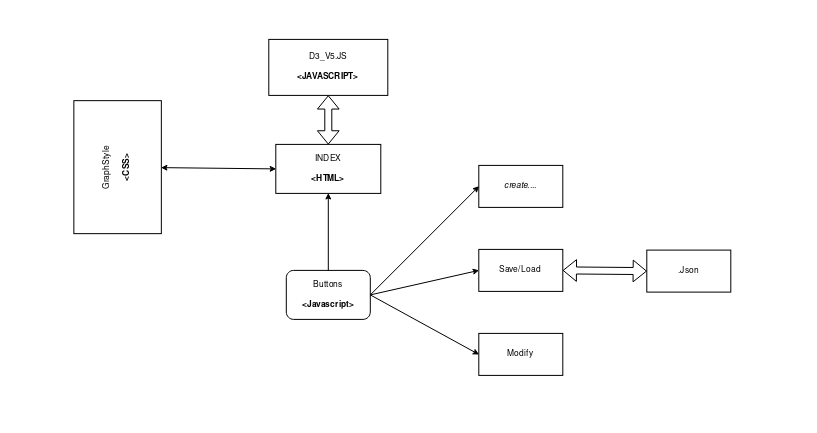
\includegraphics[width=1.2 \linewidth]{figure/primaIterazione}
	\end{center}
	\caption{Prima iterazione degli oggetti di dominio\label{fig:primaIterazione}}
\end{figure}
Come si nota la libreria D3.js è stata fin da subito pensato come punto centrare per le visualizzazioni. Per rendere la suddetta accessibile e utilizzabile in pieno si \`e scelto di dare molte funzionalità all'utente mostrando dunque le operazioni di interesse ed oltre lasciando a lui la possibilità di inserire alcune condizioni di utilizzo che saranno mostrate nel capitolo successivo. I problemi che sono stati affrontati con maggior interesse riguardano due importanti fattori: la facilit\`a di impiego e una visualizzazione che risultasse gradevole all'utente.
Durante una successiva analisi si \`e poi optato per alcune modifiche progettuali che sono mostrate nel diagramma ad oggetti di seguito in \figurename~\ref{fig:secondaIterazione} seguendo i principi espressi dal libro "UML distilled. Guida rapida al linguaggio di modellazione standard"\cite{UML:10} ed utilizzando \textbf{draw.io}, software di diagrammi online gratuito per la creazione di diagrammi di flusso, diagrammi di processo, organigrammi, ER e diagrammi di rete.
\begin{figure}[!htb]
	\begin{center}
		\hspace{-4.5 cm}
		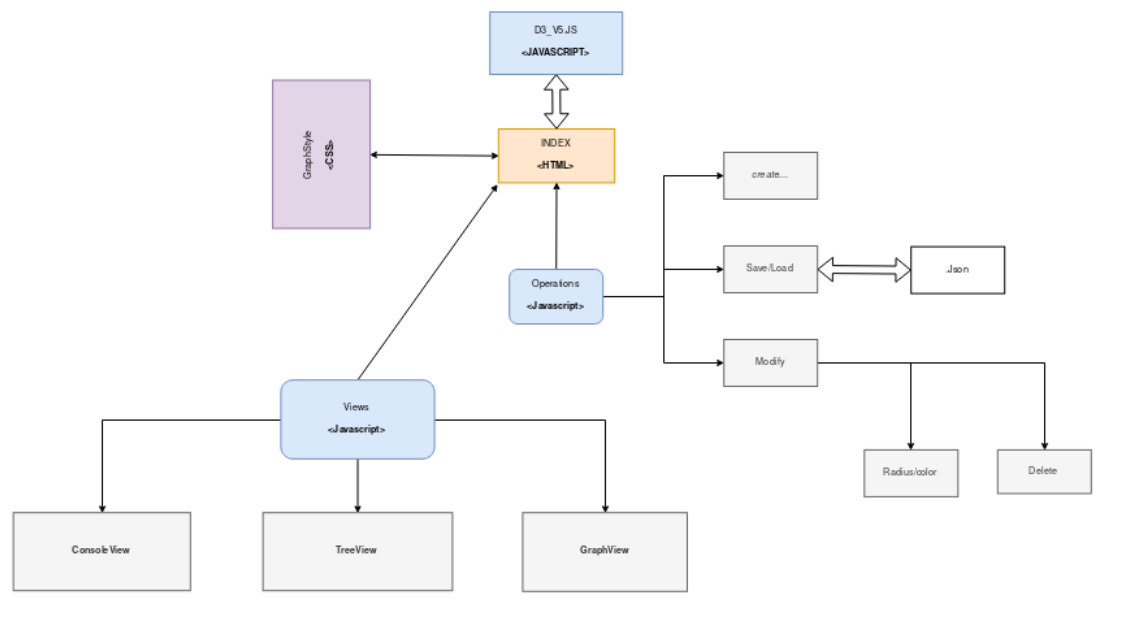
\includegraphics[width=1.2 \linewidth]{figure/secondaIterazione}
	\end{center}
	\caption{Seconda iterazione degli oggetti di dominio\label{fig:secondaIterazione}}
\end{figure}
\newpage

Nell'ingegneria del software, UML, acronimo di unified modeling language ovvero di "linguaggio di modellizzazione unificato" \`e un linguaggio di modellazione e specifica basato sul paradigma orientato agli oggetti. Il nucleo del linguaggio fu definito nel 1996 da Grady Booch, Jim Rumbaugh e Ivar Jacobson. Lo stantard \`e tuttora gestito dall'Object Management Group. UML svolge un'importantissima funzione di "lingua franca" nella comunit\`a della progettazione e programmazione ad oggetti utilizzato anche dalla gran parte della letteratura del settore informatico per descrivere soluzioni analitiche e progettuali in modo sintetico e comprensibile ad un vasto pubblico.

Tutto ci\`o che \'e stato descritto fino ad ora in questo capitolo rientra in tutta quella branca dell'informatica definita ingegneria del software che divide la creazione del progetto in tre parti distinte ma sviluppate quasi in parallelo: analisi, progettazione ed implementazione. La progettazione \`e infatti una fase del ciclo di vita del software. Sulla base della specifica dei requisiti prodotta dall'analisi, la progettazione ne definir\`a i modi in cui tali requisiti saranno soddisfatti, entrando nel merito della struttura che dovr\`a essere data al sistema software che deve essere implementato. In particolare durante il lavoro svolto \`e stata utilizzata una metodologia definita come \textbf{Agile}.
Nell'ingegneria del software, l'espressione "metodologia agile", o sviluppo agile del software, si riferisce a un insieme di metodi di sviluppo del software emersi a partire dai primi anni 2000. Di grande spunto \`e stato anche il libro "Agile Software Development: Principles, Patterns, and Practices"\cite{AG:02} I metodi agili si contrappongono al modello a cascata e altri processi software tradizionali, proponendo un approccio meno strutturato e focalizzato sull'obiettivo di consegnare al cliente, in tempi brevi e frequentemente, software funzionante e di qualit\`a.
Questi principi sono definiti nel "Manifesto per lo sviluppo agile del software"~\cite{agile2001},
pubblicato nel 2001 da Kent Beck, Robert C. Martin e Martin Fowler in cui si specificano le seguenti considerazioni:\\
\begin{center}
	\textbf{Gli individui e le interazioni} p\`u che i processi e gli strumenti\\
	\textbf{Il software funzionante} pi\`u che la documentazione esaustiva\\
	\textbf{La collaborazione col cliente} pi\`u che la negoziazione dei contratti\\
	\textbf{Rispondere al cambiamento} pi\`u che seguire un piano\\
\end{center}

Fra le pratiche promosse dai metodi agili si trovano: la formazione di team di sviluppo piccoli, poli-funzionali e auto-organizzati, lo sviluppo iterativo e incrementale, la pianificazione adattiva, e il coinvolgimento diretto e continuo del cliente nel processo di sviluppo.

\section{Principi per la visualizzazione} 
Avendo definito nel capitolo precedente la visualizzazione delle informazioni è necessario, per comprendere gli obiettivi, evidenziare i principi per una visualizzazione corretta e soprattutto il modello di progettazione.
\textbf{Tamara Macushla Munzner} propone un modello per la visualizzazione orientato al task model composto da 4 fasi:
\begin{itemize}
	\item \textbf{Dominio:} identificazione del problema e del dominio di interesse
	\item \textbf{Astrazione dei dati:} si modellano i dati che dovranno essere rappresentati
	\item \textbf{idioma di codifica:} si decide come visualizzare i dati e quali interazione implementare all'interfaccia;
	\item \textbf{Algoritmo}
\end{itemize}

Tra tutte questi principi del modello di Munzner inoltre esiste un rapporto di inclusione in cui la parte più esterna contraddistinta dal dominio a una più interna esiste un rapporto di molteplicità.
In altre parole diversi idiomi possono corrispondere alla stessa astrazione e diverse astrazioni possono corrispondere allo stesso Dominio.
Per il progetto sono stati di grande importanza i principi di Munzner e sono stati applicati con un approccio \textbf{Top-Down}, ovvero guidato dal problema e risolto dal dominio fino all'algoritmo applicando le scelte progettuali suddette.
Per quanto riguarda invece le scelte di progetto, quali ad esempio se utilizzare colori nell'interfaccia o meno, se lasciare molti spazi bianchi o utilizzare molta grafica o se utilizzare la terza dimensione o meno, anche esse sono state decise partendo dai principi chiave e di Munzner spesso in contrapposizione con quelle di Edward Rolf Tufte.\\
Per concludere la digressione sui principi della visualizzazione è importante anche definire il concetto di \textbf{User Task} come scopo dell'utente ovvero cosa l'utente deve poter fare sui dati.
Nella visualizzazione delle informazioni ci sono due principali tipi di scopi: (i)Presentazione, contesto in cui si conosce l'informazione e la visualizzazione è tesa a rappresentarla e (ii) Analisi, contesto in cui la visualizzazione è tesa all'estrazione delle informazioni dei dati rappresentati.
Per quanto concerne il progetto in questione la scelta progettuale su cui si basa è sia di presentazione che di analisi proprio per poter lasciare all'utente la possibilità di visualizzare dati senza modificarne i valori ma anche di cambiare i dati e analizzarne contenuto supportando la ricerca mediante l'automatismo delle operazioni.
}